% DONE (tsekkaa vielä kielivammaisuudet)
% --------------------------------------------------------------------
% Cheatsheet:
% \verb!lazy val!   -- esim. lyhyisiin koodinpätkiin
% \begin{verbatim}  -- esim. pitkiin koodinpätkiin
% `` tekstiä ''     -- lainausmerkit
% \textbf{huom!}    -- boldaus
% \begin{quotation}
% \noindent \it     -- quoten lisäys
% \ldots            -- kolme pistettä
% footnote{juh}     -- alaviite
% \citet, \citep
% \citet[s.234]{}   -- viitteet, http://merkel.zoneo.net/Latex/natbib.php
% \begin{sloppypar} -- ahdas teksti
% \clearpage        -- onkkelmien korjaamiseen lukujen kanssa
% --                -- yhdysviiva
% \enumerate
% \itemize          -- listat
% \begin[htb]{figure}
% \begin[htb]{table} - Kuva ja taulukko, (h)ere, (t)op, (b)ottom
% \begin{equation}  -- kaava
% \label{eq:kaava1} -- laabeli
%!TEX root = main.tex

% \subsection{Päättymättömät tietorakenteet ja kontrollirakenteet}
% 
% Jo 1980-luvun varhaisessa tutkimuksessa käsiteltiin laiskan evaluoinnin mahdollistamia laiskoja tietorakenteita, etenkin ``päättymättömiä tietorakenteita''. Näitä ovat muun muassa päättymättömät listat, puurakenteet ja tapahtumavirrat. Ne ovat tyypillisesti rekursion avulla toteutettuja, ja laiskan evaluoinnin ansiosta tietorakenteessa tarvitsee mennä vain niin ``syvälle'' kuin on tarvetta.
% 
% Eräs klassinen esimerkki on matematiikan äärettömiä lukujonojen kuvaaminen. Seuraavassa on Fibonaccin lukujono ilmaistuna rekursiivisesti Haskellilla. Huomionarvoista on, kuinka paljon koodi muistuttaa tapaa, jolla rekursiivinen lukujono ilmaistaisiin matematiikassa:
% 
% \begin{alltt}
% fib 0 = 0
% fib 1 = 1
% fib n = fib (n-1) + fib (n-2)
% \end{alltt}
%

\section{Sovellutuksia ohjelmointikielissä ja apukirjastoissa}\label{sovellutuksia}

Laiskaa evaluointia voi käyttää myös yksittäisissä kielen ominaisuuksissa. Tämä osio käy läpi, millaisia sovellutuksia laiskalle evaluoinnille on suosituissa ohjelmointikielissä. Luku on jäsennelty sovellutuksittain, jotta ohjelmointikielien väliset toteutuserot tulevat selkeästi ilmi. Sovellutukset on koottu taulukkoon \ref{table:sovellutukset}, ja alaluvuissa niitä käydään läpi tarkemmin.

\begin{table}[h]
\footnotesize
\definecolor{verylightgray}{gray}{0.95}
\begin{center}
    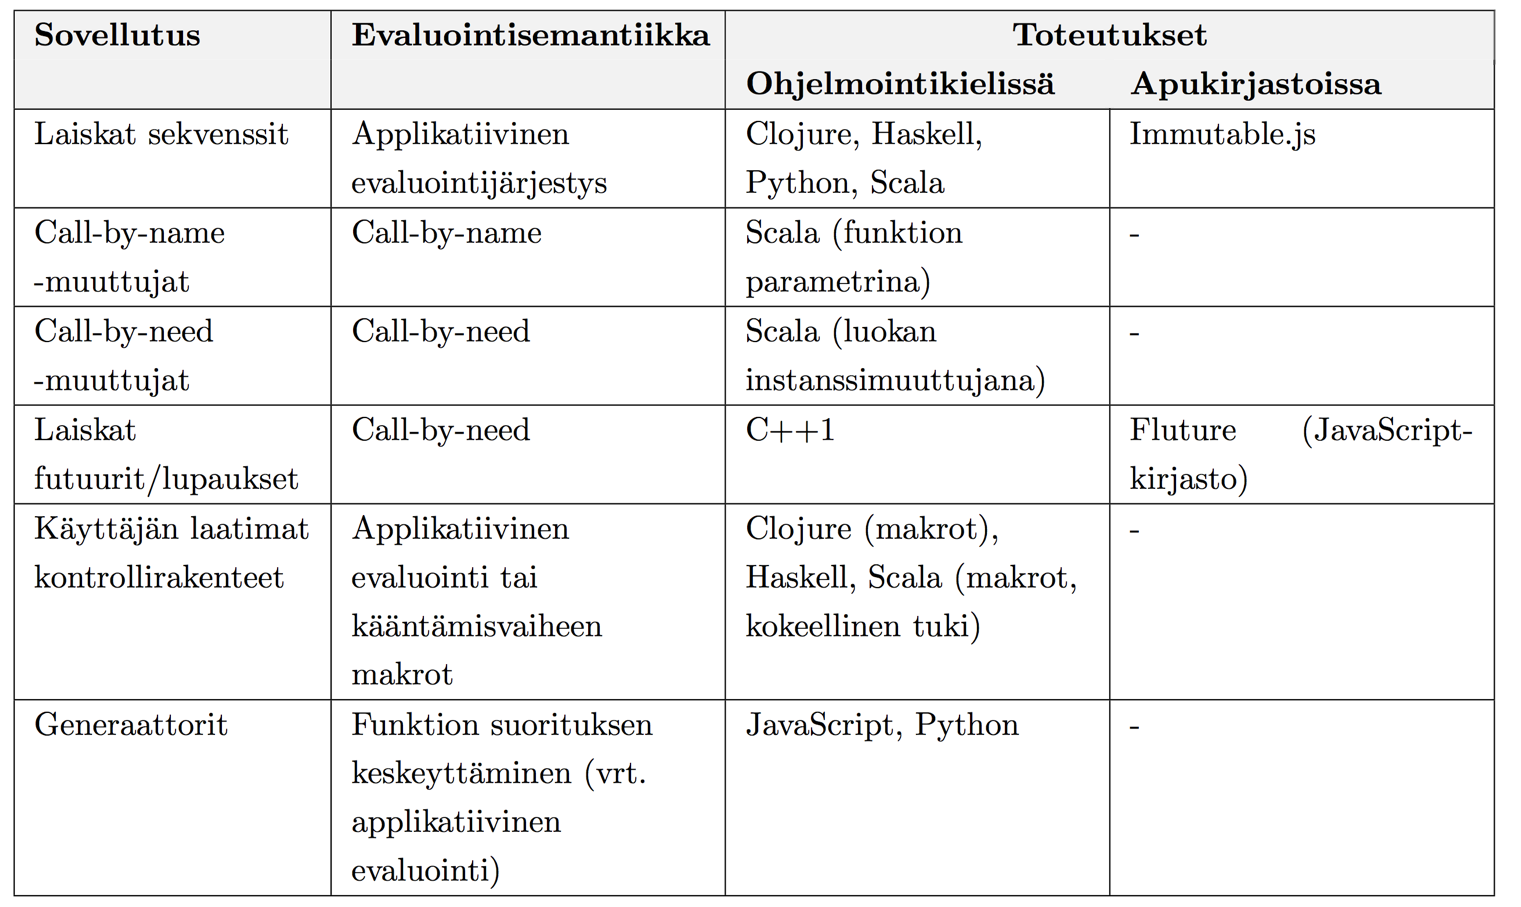
\includegraphics[width=1.0\textwidth]{applications-table}
% 	\begin{tabularx}{\linewidth}{|>{\raggedright}p{2.97cm}|>{\raggedright}p{3.8cm}|>{\raggedright}X|X|}
% 	\hline
% 	\rowcolor{verylightgray} \textbf{Sovellutus} & \textbf{Evaluointisemantiikka} & \multicolumn{2}{c}{\textbf{Toteutukset}} \\
% 	\rowcolor{verylightgray} & & \textbf{Ohjelmointikielissä} & \textbf{Apukirjastoissa}\\
% 	\hline
% 	Laiskat sekvenssit & Applikatiivinen evaluointijärjestys & Clojure, Haskell, Python, Scala & Immutable.js \\
% 	\hline
% 	Call-by-name -muuttujat & Call-by-name & Scala (funktion parametrina) & - \\
% 	\hline
% 	Call-by-need -muuttujat & Call-by-need & Scala (luokan instanssimuuttujana) & - \\
% 	\hline
% 	Laiskat futuurit/lupaukset & Call-by-need & C++1 & Fluture (JavaScript-kirjasto) \\
% 	\hline
% 	Käyttäjän laatimat kontrollirakenteet & Applikatiivinen evaluointi tai kääntämisvaiheen makrot & Clojure (makrot), Haskell, Scala (makrot, kokeellinen tuki) & - \\
% 	\hline
% 	Generaattorit & Funktion suorituksen keskeyttäminen (vrt. applikatiivinen evaluointi) & JavaScript, Python & - \\
% 	\hline
% \end{tabularx}
\end{center}
	\caption{\footnotesize \textbf{Sovellutukset koottuna.} Toteutus ohjelmointikielessä tarkoittaa, että kieli tukee sovellutusta joko syntaksinsa tai standardikirjastonsa kautta. Toteutus apukirjastossa tarkoittaa, että sovellutusta emuloidaan ohjelmointikielen tarjoamilla välineillä.}
    \label{table:sovellutukset}
\normalsize
\end{table}

\subsection{Läpikäydyt ohjelmointikielet}

Valitsin tarkasteluun viisi ohjelmointikieltä, jotka ovat keskenään erilaisia ja jotka ovat suosittuja sekä akateemisessa ympäristössä että liike-elämässä. Haskellin lisäksi valitsin seuraavat neljä kieltä:

\begin{itemize}
\item\textit{Clojure} on Lisp-kieltä muistuttava yleiskäyttöinen, funktionaalista ohjelmointityyliä tukeva ohjelmointikieli. Clojure-lähdekoodi kääntyy Java-tavukoodiksi ja on täysin yhteensopiva Java-kirjastojen kanssa.

\item \textit{JavaScript} on ainoa verkkoselainten yleisesti tukema ohjelmointikieli, ja lisäksi JavaScriptiä käytetään runsaasti myös palvelinohjelmointiin. Se tukee funktionaalista ohjelmointityyliä rajoitetusti.

\item\textit{Python} on sekä imperatiivista että rajatusti funktionaalista ohjelmointia tukeva yleiskäyttöinen ohjelmointikieli. Se on suosittu niin tieteellisessä käytössä kuin verkkokehityksessä.

\item\textit{Scala} on sekä funktionaalista että imperatiivista ohjelmointia tukeva yleiskäyttöinen ohjelmointikieli. Scala-lähdekoodi kääntyy Clojuren tapaan Java-tavukoodiksi, ja kieli on täysin yhteensopiva Java-kirjastojen kanssa.
\end{itemize}

\subsection{Laiskat sekvenssit}

\textit{Laiska sekvenssi} on listatietorakenne, joissa listan arvoja evaluoidaan sitä mukaan kun ohjelmakoodi tarvitsee niitä.

Clojure tukee laiskoja sekvenssejä, eli listamaisia tietorakenteita, joita varten kielessä on valmis tuki \verb!lazy-seq! -makron avulla. Käytännössä Clojuren käyttäjä tulee käyttäneeksi laiskoja sekvenssejä paljon, sillä monet kielen yleisimmistä listamaisten tietorakenteiden operaatioista palauttavat laiskan sekvenssin. Näitä operaatioita ovat esimerkiksi \verb!map!, \verb!filter! ja \verb!take!. Clojuren laiskojen listojen arvoja evaluoidaan sitä mukaan kuin niitä tarvitaan, ja arvot pysyvät muistissa tulevia käyttökertoja varten.

JavaScript-ohjelmointikielessä ei itsessään ole tukea laiskoille sekvensseille. Kuitenkin Facebookin julkaisema suosittu \textit{Immutable.js}-apukirjasto tarjoaa tuen funktionaaliselle ohjelmoinnille ominaisille pysyvätilaisille tietorakenteille. Kaikki kirjastossa määritellyt sekvenssit, esimerkiksi indeksoidun listan \verb!List! tai pinon \verb!Stack!, voi muuttaa laiskaksi \verb!Seq!-konstruktorilla. Sekvenssille kohdistettavat operaatiot ovat tämän luokan metodeja, ja kun \verb!Seq!-instanssille kutsuu näitä metodeja, ne palauttavat uuden laiskan sekvenssin. Ketjutetut operaatiot evaluoidaan vasta sitten, kun lopullista arvoa tarvitaan.

\begin{sloppypar}
\verb!Seq! tukee myös päättymättömiä sekvenssejä kirjaston tarjoamien \verb!Range!- ja \verb!Repeat! \mbox{-konstruktoreiden} sekä iteraattorifunktioiden avulla. \verb!Seq! ei kuitenkaan Clojuren laiskojen listojen tapaan pidä evaluoituja arvoja muistissa.
\end{sloppypar}

Myös Python tukee laiskoja sekvenssejä \textit{generaattorilausekkeiden} (eng. \textit{generator expression}) avulla ja Scalassa \textit{virtojen} (eng. \textit{stream}) avulla. Molempien kielien toteutukset ovat listarakenteisiin erikoistuneita versioita generaattoreista, joita käsitellään tarkemmin alaluvussa \ref{generaattorit}.

\subsection{Call-by-need -muuttujat}

Scala tukee \textit{call-by-need muuttujia} luokkien instanssimuuttujina. Niitä käytetään lisäämällä \verb!lazy! -avainsana instanssimuuttujan määrittelyn alkuun. Kyseisen muuttujan arvon määrittävä lauseke evaluoidaan vasta sitten, kun muuttujaa käytetään ensimmäistä kertaa. Arvo sidotaan muuttujaan, eli jos muuttujaa tarvitaan uudelleen, arvoa ei tarvitse evaluoida uudelleen.

\subsection{Call-by-name -muuttujat}

Scala tukee \textit{call-by-name -muuttujia} funktion parametreina. Ne luodaan funktion määrittelyssä syntaksilla \verb!parameterName: => Type!. Funktiokutsussa parametrin arvo evaluoidaan vasta, kun parametria käytetään. Laiskasta muuttujasta poiketen arvoa ei kuitenkaan evaluointihetkellä sidota parametriin, vaan jos parametria käytetään uudelleen, niin arvokin evaluoidaan uudelleen.

\subsection{Laiskat futuurit}
\textit{Futuuri} (eng. \textit{future}, \textit{promise} tai \textit{deferred}) tarkoittaa ohjelmointikielen rakennetta sellaisten operaatioiden kuvaamiseen, jotka voivat olla evaluoimatta, joiden evaluointi on kesken tai joiden evaluointi on jo palauttanut arvon. Futuureja käytetään operaatioiden keskinäiseen koordinoitiin ja synkronointiin.

Useimmissa ohjelmointikielissä futuurit ovat ahneita, eli niiden kuvaamaan operaation evaluointi aloitetaan futuurin luontihetkellä. \textit{Laiskat futuurit} ovat futuureja, joissa vasta se, kun ohjelmakoodi haluaa käyttää futuurin kuvaaman operaation arvoa, aiheuttaa operaation evaluoinnin.

C++ tukee laiskoja futuureja, ja niitä voi luoda kutsumalla \verb!std::async! -funktiota \verb!std::launch:deferred! -asetuksella. Funktiokutsu palauttaa palauttaa \verb!std::future! -olion, jonka \verb!get! -metodi aiheuttaa operaation suorituksen.

\subsection{Käyttäjän laatimat kontrollirakenteet}

\textit{Kontrollirakenteella} tarkoitetaan kielen natiivisyntaksin, kuten `if`, `for` tai `while`, kaltaisten rakenteiden luomisen itse. Esimerkiksi if-ehtolauseesta on Haskellissa helppoa tehdä oma versio, jossa ehdon täyttymisen perusteella evaluoidaan vain jompikumpi vaihtoehtoisista lausekkeista:

\begin{alltt}
% Käyttö: myIf condition onTrue onFalse
myIf :: Bool -> a -> a -> a
myIf True  x _ = x
myIf False _ y = y
\end{alltt}

Omien kontrollirakenteiden tuki helpottaa kieleen upotettujen \textit{täsmäkielten} rakentamista. Täsmäkielillä tarkoitetaan pieniä, tavanomaisesti deklaratiivisia kieliä, jotka ovat hyvin ilmaisuvoimaisia tietyssä ongelma-avaruudessa \citep{van2000domain}. Täsmäkielet toteutetaan usein ohjelmointikielen apukirjastoina, ja täsmäkieli on siinä tapauksessa yhdistelmä ohjelmointikielen valmiita ominaisuuksia ja apukirjastossa siihen laadittuja lisäyksiä.

Clojure puolestaan tukee \textit{makroja}, joiden avulla kielen kääntäjää pystyy laajentamaan ohjelmakoodista käsin, ja sen myötä kieleen voi luoda omia kontrollirakenteita.

\subsection{Generaattorit}\label{generaattorit}

Generaattorit ovat ohjelmointikielen rakenne, jolla funktio pystyy keskeyttämään suorituksensa ja palauttamaan arvon useasti. Tätä käytetään etenkin silmukkarakenteiden kanssa, jossa jokainen silmukan ajo tuottaa jonkin uuden arvon. Generaattorit muistuttavat läheisesti laiskaa evaluointia, koska niiden avulla pystyy esimerkiksi pyytämään listatietorakenteiden seuraavia alkioita alkio alkiolta tarpeen mukaan.

JavaScript ja Python toteuttavat generaattorit siten, että ne palauttavat \textit{iteraattorin}, jolta voi pyytää seuraavaa arvoa. Myös kielten listarakenteet noudattavat iteraattorirajapintaa, joten sen myötä listoja ja generaattoreilla luotuja iteraattoreita voi käsitellä monilla samoilla komennoilla.